\section{\acs{cocomo} Approach} \label{sec:cocomo}
%Apply COCOMO to estimate effort and cost.

In this section of the document, we are going to apply the \acs{cocomo} approachin order to estimate effort and cost for our project.
In order to do that, we are going to refer to the \acs{cocomo} II model definition manual at the following link: \url {http://csse.usc.edu/csse/research/COCOMOII/cocomo2000.0/CII_modelman2000.0.pdf}.

\begin{table}[htbp]
\begin{center}
\begin{tabular}[t]{ccc}

\hline
\textbf{Scale Driver} & \textbf{Factor} & \textbf{Value} \\
\hline
\acs{prec} & \texttt{High} &  $2.48$\\
\hline
\acs{flex} & \texttt{Nominal} & $3.04$\\
\hline
\acs{resl}&  \texttt{Low} &  $5.65$\\
\hline
\acs{team} & \texttt{High} &  $2.19$\\
\hline
\acs{pmat} & \texttt{High} & $3.12$ \\
\hline

\end{tabular}
\caption{Scale drivers and the corresponding Factor and Value}
\end{center}
\end{table}

We considered the following scale drivers:

\begin{itemize}

\item[\textbf{--}] \textit{\acl{prec}}: if a product is similar to several previously developed projects, then \acs{prec} is high. Since on the market there are already some project similar to our, we rate this scale driver as \texttt{High}, with a corresponding value of $2.48$

\item[\textbf{--}] \textit{\acl{flex}}: if there are no specific constraints to conform to pre-established requirements and external interface specifications, then \acs{flex} is high. Since we had to remain compliance with the specification given, but with some relaxation for some of the specifications, we rate this scale driver as \texttt{Nominal}, with a corresponding value of $3.04$

\item[\textbf{--}] \textit{\acl{resl}}: if we have a good risk management plan, clear definition of budget and schedule, focus on architectural definition, then \acs{resl} is high. Since it is the first time we have to manage a project, we are not too confident about the precision of our Risk Management Plan, Scheduling and Resource Allocation. So, we rate this scale driver as \texttt{Low}, with a corresponding value of $5.65$

\item[\textbf{--}] \textit{\acl{team}}: if all stakeholders are able to work in a team and share the same vision and commitment, then \acs{team} is high. In these past months our team worked very well together, but we think that the external stakeholders may have a vision different (even a little) from ours.
For this reason, we rate this scale driver as \texttt{High}, with a corresponding value of $2.19$

\item[\textbf{--}] \textit{\acl{pmat}}: in order to rate this driver, we have to refers to a well known method for assessing the maturity of a software organization, that is \acs{cmmi}. We can estimate that our project is at \texttt{Maturity Level 3 - Defined}, that correponds to a \acs{pmat} at level \texttt{High} and a value of $3.12$.

\end{itemize}

Notice that while the \acs{prec} and \acs{flex} scale factors are largely intrinsic to a project and uncontrollable, the following three scale factors identify management controllables by which projects can reduce diseconomies of scale by reducing sources of project turbulence, entropy, and rework.

\begin{table}[htbp]
\begin{center}
\begin{tabular}[t]{ccc}

\hline
\textbf{Cost Driver} & \textbf{Factor} & \textbf{Value} \\
\hline
\acs{rely} & \texttt{Nominal} &  $1.00$\\
\hline
\acs{data} & \texttt{Nominal} & $1.00$\\
\hline
\acs{cplx}&  \texttt{Nominal} &  $1.00$\\
\hline
\acs{ruse} & \texttt{High} &  $1.07$\\
\hline
\acs{docu} & \texttt{High} & $1.11$ \\
\hline
\acs{time} & \texttt{Nominal} & $1.00$ \\
\hline
\acs{stor} & \texttt{Nominal} & $1.00$ \\
\hline
\acs{pvol} & \texttt{Nominal} & $1.00$ \\
\hline
\acs{acap} & \texttt{Nominal} & $1.00$ \\
\hline
\acs{pcap} & \texttt{Nominal} & $1.00$\\
\hline
\acs{pcon} & \texttt{Very High} & $0.81$ \\
\hline
\acs{apex} & \texttt{Low} & $1.10$ \\
\hline
\acs{plex} & \texttt{Very Low} & $1.19$ \\
\hline
\acs{ltex} & \texttt{Low} & $1.09$ \\
\hline
\acs{tool} & \texttt{Nominal} & $1.00$ \\
\hline
\acs{site} & \texttt{Low} & $1.09$ \\
\hline
\acs{sced} & \texttt{Nominal} & $1.00$ \\
\hline

\end{tabular}
\caption{Cost drivers and the corresponding Factor and Value}
\end{center}
\end{table}

\begin{itemize}

\item[\textbf{--}] \textbf{Product factors}: they account for variation in the effort required to develop software caused by characteristics of the product under development. A product that is complex, has high reliability requirements, or works with a large testing database will require more effort to complete. There are five product factors, and complexity has the strongest influence on estimated effort.

\begin{itemize}
	
	\item \textit{\acl{rely}}: this is the measure of the extent to which the software must perform its intended function over a period of time. If the effect of a software failure is only slight inconvenience then \acs{rely} is very low. If a failure would risk human life then \acs{rely} is very high. In our case, we think that the appropriate rate for this driver is \texttt{Nominal}, with a corresponding value of $1.00$.
	
	\item \textit{\acl{data}}: this cost driver attempts to capture the effect large test data requirements have on product development. \acs{data} is capturing the effort needed to assemble and maintain the data required to complete test of our program. In our case, we can estimate that the rate for this driver is \texttt{Nominal}, with a corresponding value of $1.00$.
	
	\item \textit{\acl{cplx}}: complexity is divided into five areas: control operations, computational operations, device-dependent operations, data management operations, and user interface management operations.  Basing on this, we can estimate that the rate for this driver is \texttt{Nominal}, with a corresponding value of $1.00$.
	
	\item \textit{\acl{ruse}}: this cost driver accounts for the additional effort needed to construct components intended for reuse on current or future projects. This effort is consumed with creating more generic design of software, more elaborate documentation, and more extensive testing to ensure components are ready for use in other applications. In our case, we can estimate that the rate for this driver is \texttt{High}, with a corresponding value of $1.07$.
	
	\item \textit{\acl{docu}}: this cost driver is about the level of required documentation. The rating scale for this cost driver is evaluated in terms of the suitability of the project's documentation to its life-cycle needs. The rating scale goes from \texttt{Very Low}, if many life-cycle needs are left uncovered, to \texttt{Very High}, if the documentation is very excessive for life-cycle needs). In our case, we can estimate that the rate for this driver is \texttt{High}, with a corresponding value of $1.11$
	
	\end{itemize}
	
\item[\textbf{--}] \textbf{Platform factors}: the platform refers to the target-machine complex of hardware and infrastructure software. The factors have been revised and some additional platform factors were considered, such as distribution, parallelism, embeddedness, and real-time operations.

	\begin{itemize}
	
	\item \textit{\acl{time}}: this is a measure of the execution time constraint imposed upon a software system. The rating is expressed in terms of the percentage of available execution time expected to be used by the system or subsystem consuming the execution time resource. The rating ranges from \texttt{Nominal}, less than $50\%$ of the execution time resource used, to \texttt{Extra High}, when $95\%$ of the execution time resource is consumed. In our case, we can estimate that the rate for this driver is \texttt{Nominal}, with a corresponding value of $1.00$
	
	\item \textit{\acl{stor}}: this rating represents the degree of main storage constraint imposed on a software system or subsystem. The rating ranges from \texttt{Nominal}, less than $50\%$ , to \texttt{Extra High}, whan  $95\%$. In our case, we can estimate that the rate for this driver is \texttt{Nominal}, with a corresponding value of $1.00$
	
	\item \textit{\acl{pvol}}: "platform" is used here to mean the complex of hardware and software (\acs{os}, \acs{dbms}, etc.) the software product calls on to perform its tasks. This rating ranges from \texttt{Low}, where there is a major change every 12 months, to \texttt{Very High}, where there is a major change every two weeks. In our case, we can estimate that the rate for this driver is \texttt{Nominal}, with a corresponding value of $1.00$
	
	\end{itemize}
	
\item[\textbf{--}] \textbf{Personnel Factors}: after product size, people factors have the strongest influence in determining the amount of effort required to develop a software product. These factors are for rating the development team's capability and experience, not the individual. 

\begin{itemize}
	
	\item \textit{\acl{acap}}: analysts are personnel who work on requirements, high-level design and detailed design. The major attributes that should be considered in this rating are analysis and design ability, efficiency and thoroughness, and the ability to communicate and cooperate. Analyst teams that fall in the fifteenth percentile are rated \texttt{Very Low} and those that fall in the ninetieth percentile are rated as \texttt{Very High}.  In our case, we can estimate that the rate for this driver is \texttt{Nominal}, with a corresponding value of $1.00$
		
	\item \textit{\acl{pcap}}: Current trends continue to emphasize the importance of highly capable analysts. However, we have a trend toward higher importance of programmer capability as well.
Evaluation should be based on the capability of the programmers as a team rather than as individuals. Major factors which should be considered in the rating are ability, efficiency and thoroughness, and the ability to communicate and cooperate. A \texttt{Very Low} rated programmer team is in the fifteenth percentile and a \texttt{Very High} rated programmer team is in the ninetieth percentile. In our case, we can estimate that the rate for this driver is \texttt{Nominal}, with a corresponding value of $1.00$

	\item \textit{\acl{pcon}}: the rating for this cost driver is in terms of the project's annual personnel turnover: from 3\%, very high continuity, to 48\%, very low continuity. In our case, we can estimate that the rate for this driver is \texttt{Very High}, with a corresponding value of $0.81$
	
	\item \textit{\acl{apex}}: the rating for this cost driver is dependent on the level of applications experience of the project team developing the software system or subsystem. The ratings are defined in terms of the project team's equivalent level of experience with this type of application. A \texttt{Very Low} rating is for application experience of less than 2 months. A very \texttt{Very High} is for experience of 6 years or more. In our case, we can estimate that the rate for this driver is \texttt{Low}, with a corresponding value of $1.10$
	
	\item \textit{\acl{plex}}: the Post-Architecture model broadens the productivity influence of platform experience by recognizing the importance of understanding the use of more powerful platforms, including more graphic user interface, database, networking, and distributed middleware capabilities. In our case, we can estimate that the rate for this driver is \texttt{Very Low}, with a corresponding value of $1.19$.
	
	\item \textit{\acl{ltex}}: this is a measure of the level of programming language and software tool experience of the project team developing the software system or subsystem. Software development includes the use of tools that perform requirements and design representation and analysis, configuration management, document extraction, library management, program style and formatting, consistency checking, planning and control, etc. In addition to experience in the project's programming language, experience on the project's supporting tool set also affects development effort. A \texttt{Very Low} rating is given for experience of less than 2 months. A \texttt{Very High} rating is given for experience of 6 or more years.  In our case, we can estimate that the rate for this driver is \texttt{Low}, with a corresponding value of $1.09$.
		\end{itemize}
		
\item[\textbf{--}] \textbf{Project Factors}: these factors account for influences on the estimated effort such as use of modern software tools, location of the development team, and compression of the project schedule.

	\begin{itemize}
	
	\item \textit{\acl{tool}}: the tool rating ranges from simple edit and code, \texttt{Very Low}, to integrated life-cycle management tools, \texttt{Very High}. In our case, we can estimate that the rate for this driver is \texttt{Nominal}, with a corresponding value of $1.00$.
	
\item \textit{\acl{site}}: the rate of this cost driver involves the assessment and judgement-based averaging of two factors: site collocation (from fully collocated to international distribution) and communication support (from surface mail and some phone access to full interactive multimedia). In our case, we can estimate that the rate for this driver is \texttt{Low}, with a corresponding value of $1.09$.
	
	\end{itemize}
	
\item[\textbf{--}] \textbf{General Factor}

	\begin{itemize}
	
	\item \textit{\acl{sced}}: this rating measures the schedule constraint imposed on the project team developing the software. The ratings are defined in terms of the percentage of schedule stretch-out or acceleration with respect to a nominal schedule for a project requiring a given amount of effort. Accelerated schedules tend to produce more effort in the earlier phases to eliminate risks and refine the architecture, more effort in the later phases to accomplish more testing and documentation in parallel. Schedule compression of 75\% is rated \texttt{Very Low}. A schedule stretch-out of 160\% is rated \texttt{Very High}. Stretch-outs do not add or decrease effort. Their savings because of smaller team size are generally balanced by the need to carry project administrative functions over a longer period of time. n our case, we can estimate that the rate for this driver is \texttt{Nominal}, with a corresponding value of $1.0$.
	
	\end{itemize}

\end{itemize}

In the second phase of the estimation analysis, we used an online calculator in order to compute the effort, the total cost, the duration and the number of person estimated for the completion of our project.
You can find the online calculator that we used at the following link: \url{http://csse.usc.edu/tools/COCOMOII.php}.

\begin{figure}[htbp]
\centering
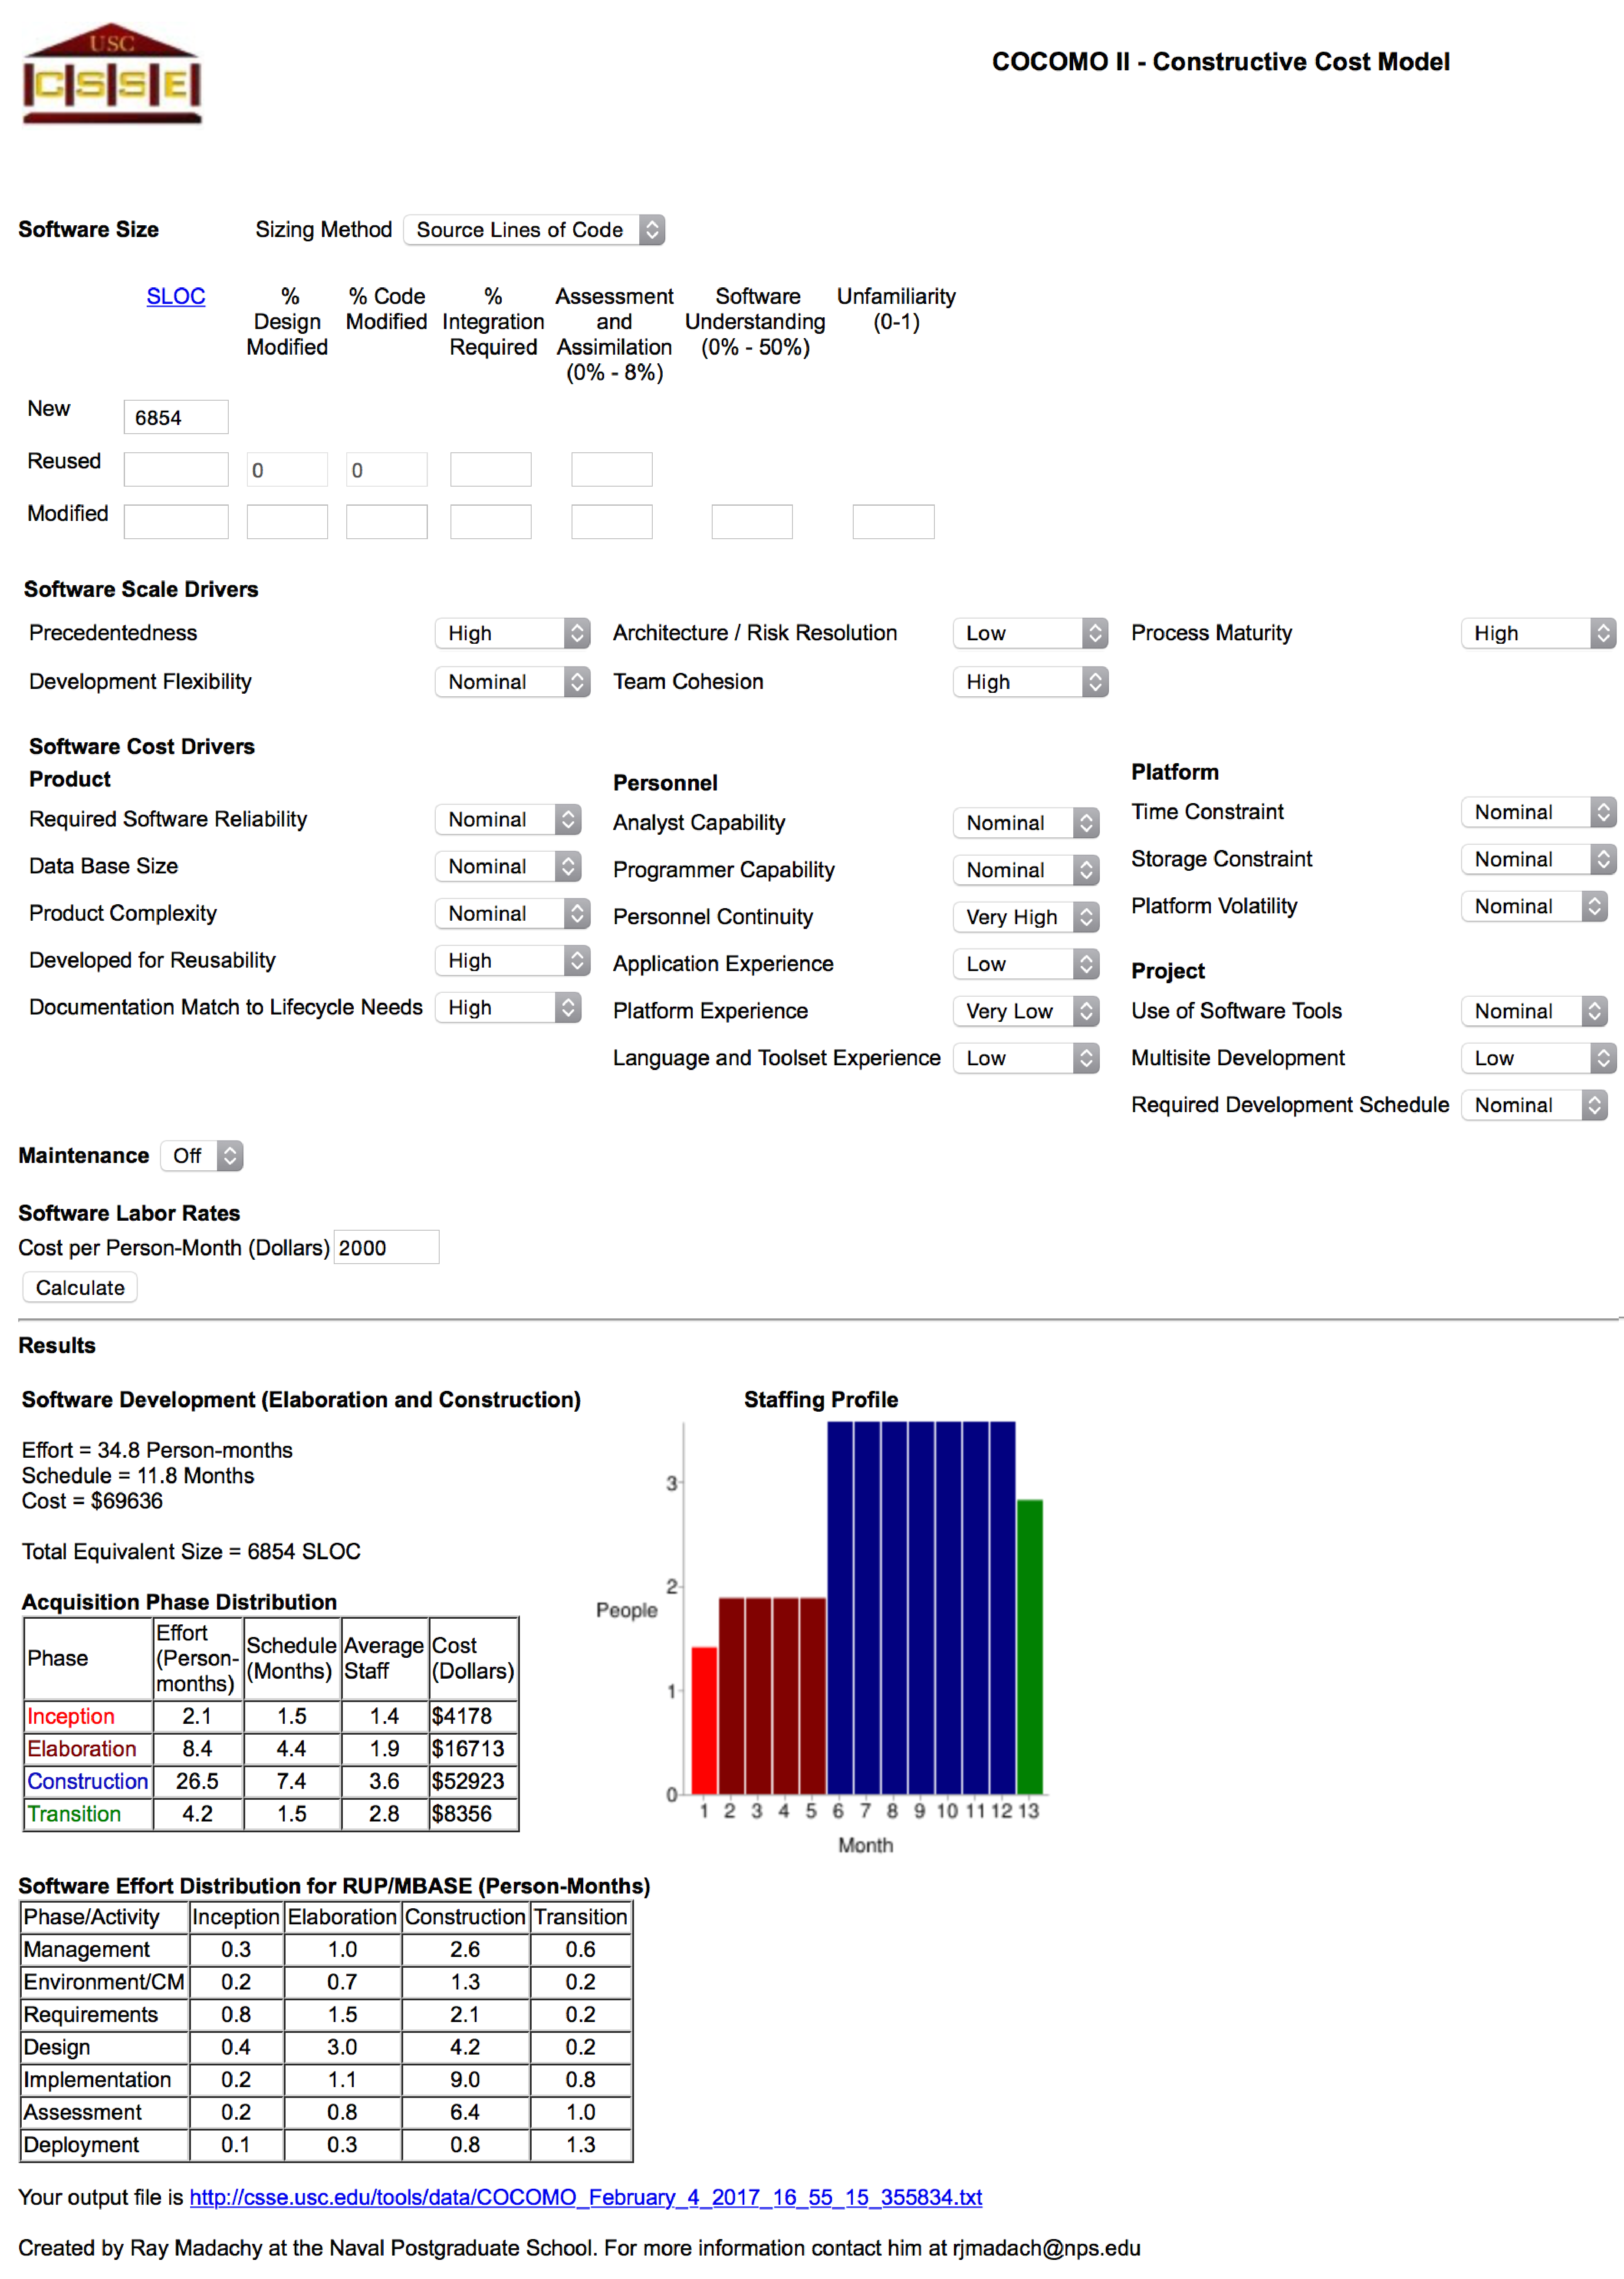
\includegraphics[width=\textwidth]{Images/cocomo_v1}
\caption{Grafical representation of effort, total cost, duration and number of person estimated for the completion of our project}
\label{fig:chart}
\end{figure}

\clearpage

In conclusion, we calculated this value for \textbf{effort}, \textbf{total cost}, \textbf{duration} and \textbf{team size}:

\begin{itemize}

\item[\textbf{--}] \textbf{Effort}: $28.2$ Person-months
\item[\textbf{--}] \textbf{Total Cost}: $\$56386$, if we consider an average cost equals to $\$2000$ per Person-months
\item[\textbf{--}] \textbf{Duration}: $11.0$ Months
\item[\textbf{--}] \textbf{Team Size}: \[\frac{\textbf{Effort}}{\textbf{Duration}} = \frac{28.2}{11.0} = 2.56\:members\] 

\end{itemize}